\section{Sprache}

\subsection{Typenmodell}
\label{subsec:Typenmodell}
\subsubsection{Objekte}
\label{subsubsec:Objekte}
Objekte sind Instanzen, die Werte eines gegebenen Typs enthalten. Das umfasst sowohl Objekte im Sinn der objektorientierten Programmierung wie auch einfache Instanzen. Objekte werden allgemein durch Objektdeklarationen deklariert, aber auch formale Parameter von Unterprogrammen und loop-Parameter werden als Objekte behandelt. Ebenso sind Komponenten von Objekten auch Objekte.\\
Objekte sind entweder Variablen oder Konstanten. Konstanten müssen initialisiert werden und auch der Wert von Variablen muss zur Zeit der Kompilierung bekannt sein.\\
\begin{lstlisting}[caption={Beispiele für einfache Objekte in Spark}, label=spark:einfacheObjekte]
Count, Sum: Integer;
Sorted: Boolean := False;
Limit: constant Integer := 10_1000;
Level: constant Float := 3.5;
\end{lstlisting}


Es ist nicht möglich bei der Objektdeklaration einen expliziten Constraint anzugeben. Das heißt, dass der (Sub-)Typ eines Objektes immer mit dem Schlüsselwort \texttt{subtype} und nicht nur durch einen Subtypindikator festgelegt wird.

\begin{lstlisting}[caption={Deklaration gültig in Ada, aber unzulässig in Spark}, label=ada:falscheDeklarationinAda]
I, J, K: Integer range 1 .. 10;
\end{lstlisting}

\begin{lstlisting}[caption={korrekte Deklaration in Spark}, label=spark:korrekteDeklarationinSpark]
subtype Index is Integer range 1 .. 10;
I, J, K: index;
\end{lstlisting}


Listing~\ref{spark:korrekteDeklarationinSpark} zeigt, dass alle Objekte in \texttt{Spark} benannte Subtypen haben müssen(außer loop-Parametern).

%TODO later layoutcheck for free page
\newpage

\subsubsection{Typen und Subtypen}
\label{subsubsec:TypenUndSubtypen}

\begin{figure}[h!]
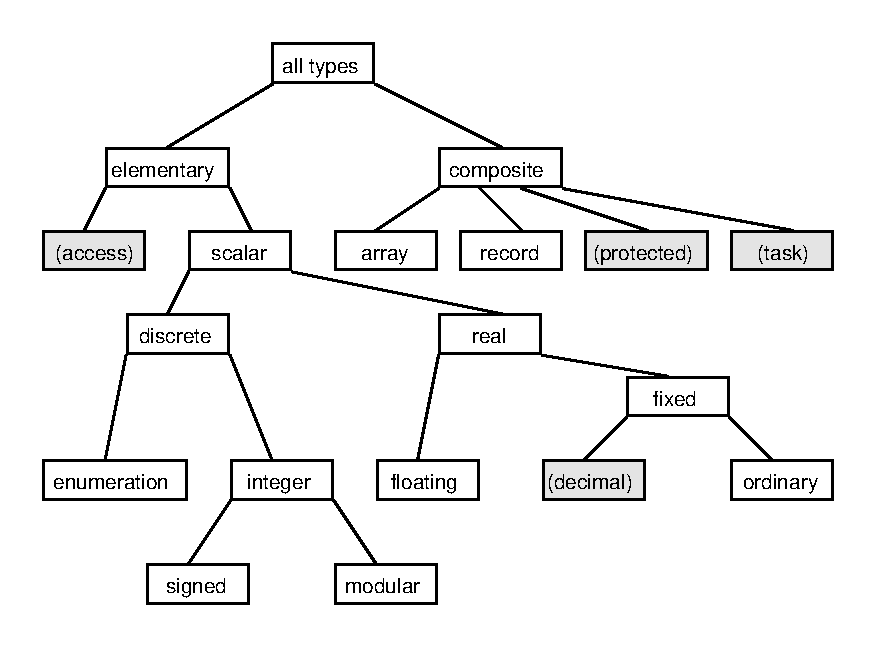
\includegraphics[width=\textwidth{}]{images/typeHierarchy.pdf}
\label{fig:typeHierarchy}
\caption{Hierarchie der Typen in Ada und Spark}
\end{figure}

Abbildung~\ref{fig:typeHierarchy} zeigt die verfügbaren Typen in \texttt{Ada} und mit grauer Hinterlegung bzw. in Klammern geschrieben die in \texttt{Spark} nicht verfügbaren Typen: \textit{access}, \textit{protected}, \textit{task} und \textit{decimal}.\\
Die in \texttt{Spark} vordefinierten Typen sind:\\
enumeration:
\begin{itemize}
	\item Boolean
	\item Character
\end{itemize}
fixed point type:
\begin{itemize}
	\item Duration
\end{itemize}
integer:
\begin{itemize}
	\item Integer
	\item Long\_Integer
\end{itemize}
float:
\begin{itemize}
	\item Float
	\item Long\_Float
\end{itemize}
array:
\begin{itemize}
	\item String
\end{itemize}

Weitere Typen können wie in \texttt{Ada} deklariert werden, jedoch mit gewissen Einschränkungen.\\
\textit{Ranges} müssen \textit{statisch} sein, also ihre Größe zur Kompilierung bekannt sein. Es können dazu also keine Variablen oder Funktionen verwendet werden. Da \textit{constraints} in \texttt{Spark} immer statisch sein müssen, sind auch ihre Attribute \textit{Last} und \textit{First} statisch und können verwendet werden(Listing~\ref{spark:Range constraint}).

\begin{lstlisting}[caption={Range constraint}, label=spark:Range constraint]
subtype Color is Colour range Colour'First .. Colour'Last;
\end{lstlisting}

Möchte man nur eine Umbenennung eines Typen vornehmen, so kann auch eine Kurzform verwendet werden(Listing~\ref{spark:Range constraint short}). Das ist aber nur für \textit{scalar}-Typen zulässig und nicht für \textit{private}-Typen.

\begin{lstlisting}[caption={Range constraint kurz}, label=spark:Range constraint short]
subtype Color is Colour;
\end{lstlisting}

Im Gegensatz zu \texttt{Ada} darf eine \textit{static range} in \texttt{Spark} niemals \textit{null} bzw. \textit{empty} sein, d.h. Die obere Grenze muss größer oder gleich der unteren sein(\textit{null ranges} in \textit{loops} sind erlaubt).

\begin{lstlisting}[caption={Typ des subtyps}, label=spark:Typ des subtyps]
type Colour is (White, Red, Yellow, Green, Blue, Brown);
subtype Rainbow is Colour range Red .. Blue;
R: Rainbow;
\end{lstlisting}

Zu Listing~\ref{spark:Typ des subtyps} ist wichtig, dass der Typ von \textit{R} immer noch \textit{Colour} ist.



\subsubsection{Enumaration Typen}
\label{subsubsec:EnumarationTypen}
Um die Mehrdeutigkeit zu reduzieren ist es in \texttt{Spark} nicht möglich \textit{literale} im selben \textit{scope} zu überladen. Listing~\ref{spark:literaleUeberladen} zeigt solch eine ungültige Überladung, welche in \texttt{Ada} möglich ist, in \textit{Spark} jedoch nicht möglich ist, da das \textit{literal} \textsc{Sun} in beiden Typen verwendet wird.

\begin{lstlisting}[caption={Literale überladen}, label=spark:literaleUeberladen]
type day is (Mon, Tue, Wed, Thu, Fri, Sat, Sun);
type SolarSystem is (Sun, Mercury, Venus, Earth);
\end{lstlisting}

Die aus \texttt{Ada} bekannten Vergleichsoperatoren und Attribute von \textit{enumerations} finden ihre normale Anwendung in Bezug auf ihre Reihenfolge bei der Deklaration. Sie beziehen sich aber auf den zu Grunde liegenden Typ. So ergibt \textsl{Rainbow'Succ(x)} das selbe wie \textsl{Colour'Succ(x)} auch wenn \textsl{x = blue}. Das führt dazu, dass keine eigenen character Typen deklariert werden können.\\
Der Typ \textit{Boolean} ist auch ein \textit{Enumaration} Typ, unterliegt in \texttt{Spark} aber besonderen Beschränkungen. Vergleichsoperatoren außer der (Un-)Gleihiet funktionieren nicht. Die Attribute \textit{Pred},\textit{Succ}, \textit{Pos} und \textit{Val} können nicht verwendet werden, aber \textit{First} und \textit{Last}. \textit{Boolean}s können als \textit{array index type} verwendet werden jedoch nicht als explizite \textit{range}. Verdeutlicht wird dies in Listing~\ref{spark:Boolean}.

\begin{lstlisting}[caption={Boolean}, label=spark:Boolean]
subtype ValveOpen is Boolean;  --erlaubt
subtype ValveOpen is Boolean range Boolean'First .. Boolean'Last; --falsch
subtype Always is Boolean range True .. True --falsch
\end{lstlisting}

Die Operationen \textit{and}, \textit{or}, \textit{xor} und \textit{not} haben ihre normale Bedeutung, wobei ein \textit{xor} einem \textit{/=} entspricht. 


\subsubsection{composite Typen}
\label{subsubsec:compositeTypen}
Es darf immer nur \textbf{ein} von einem \textit{tagged type} abgeleiteten Typen pro \textit{package} geben. Deswegen darf von den Deklarationen in Listing~\ref{spark:compositeTagged} immer nur eine je \textit{Package} stehen. Dadurch soll Überladung verhindert werden. Die entsprechenden Deklarationen können aber in Kindpaketen geschehen.

\begin{lstlisting}[caption={tagged types}, label=spark:compositeTagged]
type object is tagged
	record
		XCoord,YCoord: Float;
	end record;

type point is new Object with null record;

type Circle is new Object with
	record
		Radius: Float;
	end record;
\end{lstlisting}

\textit{Records} können, ebenso wie Objekte, keine \textit{constraints} enthalten. Ebenso können keine default-Werte vergeben werden. \textit{Records} in \texttt{Spark} sind daher recht einfach gestaltet und haben z.B. keine Diskriminanten.\\
\\
Auch \textit{Arrays} unterliegen den typischen Konventionen von \texttt{Spark}, dass jeder Typ benannt werden muss. Listing~\ref{spark:illegalArrays} zeigt in \texttt{Spark} ungültige Deklarationen von \textit{Arrays}, welche in Listing~\ref{spark:legalArrays} konform zu \texttt{Spark} gezeigt sind.

\begin{lstlisting}[caption={illegal Arrays}, label=spark:illegalArrays]
type Triple is array (1 .. 3) of Real;---falsch

UpperCaseTable: array(1 .. 10) of Character range 'A' .. 'Z';--falsch

NextLine:String(1 .. 80):--falsch
\end{lstlisting}
\begin{lstlisting}[caption={legal Arrays}, label=spark:legalArrays]
type Tuple is array (Integer range <>) of Real;
subtype TripleIndex is Integer range 1 .. 3;
subtype Triple is Tuple(TripelIndex);

subtype Index is Integer range 1 .. 10;
subtype CapitalLetter is Character range 'A' .. 'Z';
type UpperCaseArray is array (Index) of CapitalLetter;
UpperCaseTable: UpperCaseArray;

subtype LineIndex is Integer range 1 .. 80;
subtype Line is String(LineIndex);
NextLine: Line;
\end{lstlisting}

Alle \textit{constraints} in \texttt{Spark} sind \textit{statisch}, haben also \textit{statische Grenzen}, was dazu führt, dass in \texttt{Spark} keine Arrays deklariert werden können, deren Grenzen nicht zur Programmausführung bekannt sind.
Es gibt keinen \textit{slices} von \textit{arrays} in \texttt{Spark} ebenso ist \textit{sliding} nicht möglich.


\subsubsection{Aggregate}
\label{subsubsec:Aggregate}

\begin{lstlisting}[caption={illegal Aggregates}, label=spark:illegalAggregates]
Z:Complex:=(0.0,0.0);--falsch
Z:Complex:=(Re | Im => 0.0);--falsch
Z:Complex:=(others => 0.0);--falsch
\end{lstlisting}
\begin{lstlisting}[caption={legal Aggregates}, label=spark:legalAggregates]
Z:Complex:=Complex'(0.0,0.0);
Z:Complex:=Complex'(Re => 0.0,Im => 0.0);
\end{lstlisting}

\subsubsection{Ausdrücke}
\label{subsubsec:Ausdruecke}
Ausdrücke beschreiben die Berechnung eines Wertes. Da \texttt{Spark} keine Überladung kennt(außer den vordefinierten Operationen wie +), gibt es keine Notwendigkeit zur Auflösung einer Überladung und der Typ eines Ausdrucks ist bestimmt durch die Typen seiner Bestandteile und der Operatoren und nicht durch den Kontext. Im Allgemeinen sind Ausdrücke in \texttt{Spark} denen aus \texttt{Ada} sehr ähnlich, mit ein paar Ausnahmen,\\
Die möglichen Operatoren sind in aufsteigender Priorität:
\begin{itemize}
	\item logische Operatoren: \textit{and, or, xor} zzgl. $and then, or else$
	\item realtionale operatoren: $=, /=, <, <=,> ,>=$ zzgl. $in, not in$
	\item binär additive Operatoren: $+, - , \&$
	\item unär additive Operatoren: $+, -$
	\item multiplicative Operatoren: $*, /, mod, rem$
	\item höchste Priorität: $**, abs, not$
\end{itemize}
Wie schon erwähnt ist in \texttt{Spark} kein \textit{sliding} möglich. \textit{Ordnungsrelationen} können in \texttt{Spark} nicht auf \textit{Boolean} angewandt werden, ebenso nicht auf \textit{eindimensionale Array} von \textit{diskreten Typen}. Beides ist in \texttt{Ada} möglich. \textit{Strings} bilden hier aber eine Ausnahme in \texttt{Spark}.\\
\textit{Unäre Operatoren} können in \texttt{Spark} auf alle \textit{numerischen Typen} angewandt werden, nicht jedoch auf \textit{modulare}, das selbe gilt für Operatoren höchster Ordnung.


\subsubsection{Konstanten und statische Ausdrücke}
\label{subsubsec:Konstanten und statische Ausdruecke}
Objekte, welche als Konstanten deklariert werden, müssen initialisiert werden, mit einem Ausdruck, dessen Wert zur Ausführungszeit bekannt ist. Ein konstanter Ausdruck ist jeder Ausdruck, der der \textbf{keines} der folgenden enthält:

\begin{itemize}
	\item einen Variablennamen
	\item einen Funktionsaufruf(außer den vordefinierten Operatoren/Attributen)
	\item eine Komponente mit Index
	\item eine Komponete, die einen record darstellt
\end{itemize}

In \texttt{Ada} in konstant gleichzusetzen mit \textit{read only}, wohingegen in \texttt{Spark} der Wert der konstanten Feststehen muss. 

